\documentclass{article}
\usepackage[utf8x]{inputenc}
\usepackage{ucs}
\usepackage{amsmath} 
\usepackage{amsfonts}
\usepackage{upgreek}
\usepackage[english,russian]{babel}
\usepackage{graphicx}
\usepackage{float}
\usepackage{textcomp}
\usepackage{hyperref}
\usepackage{geometry}
  \geometry{left=2cm}
  \geometry{right=1.5cm}
  \geometry{top=1cm}
  \geometry{bottom=2cm}
\usepackage{tikz}
\usepackage{ccaption}
\usepackage{multicol}

\usepackage{listings}
%\setlength{\columnsep}{1.5cm}
%\setlength{\columnseprule}{0.2pt}


\begin{document}
\pagenumbering{gobble}

\lstset{
  language=C++,                % choose the language of the code
  basicstyle=\linespread{1.1}\ttfamily,
  columns=fixed,
  fontadjust=true,
  basewidth=0.5em,
  keywordstyle=\color{blue}\bfseries,
  commentstyle=\color{gray},
  stringstyle=\ttfamily\color{orange!50!black},
  showstringspaces=false,
  %numbers=false,                   % where to put the line-numbers
  numbersep=5pt,
  numberstyle=\tiny\color{black},
  numberfirstline=true,
  stepnumber=1,                   % the step between two line-numbers.        
  numbersep=10pt,                  % how far the line-numbers are from the code
  backgroundcolor=\color{white},  % choose the background color. You must add \usepackage{color}
  showstringspaces=false,         % underline spaces within strings
  captionpos=b,                   % sets the caption-position to bottom
  breaklines=true,                % sets automatic line breaking
  breakatwhitespace=true,         % sets if automatic breaks should only happen at whitespace
  xleftmargin=.2in,
  extendedchars=\true,
  keepspaces = true,
}
\lstset{literate=%
   *{0}{{{\color{red!20!violet}0}}}1
    {1}{{{\color{red!20!violet}1}}}1
    {2}{{{\color{red!20!violet}2}}}1
    {3}{{{\color{red!20!violet}3}}}1
    {4}{{{\color{red!20!violet}4}}}1
    {5}{{{\color{red!20!violet}5}}}1
    {6}{{{\color{red!20!violet}6}}}1
    {7}{{{\color{red!20!violet}7}}}1
    {8}{{{\color{red!20!violet}8}}}1
    {9}{{{\color{red!20!violet}9}}}1
}

\title{Семинар \#7: Move-семантика и умные указатели. \vspace{-5ex}}\date{}\maketitle

\section*{Копирование и перемешение}
Помимо операции копирования в \texttt{C++} есть ещё операция перемещения. Эту операцию можно применять к объектам большинства типов. Рассмотрим различие копирования и перемещения на следующем примере. Пусть у нас есть объект \texttt{a} некоторого типа \texttt{Type}, находящийся в состоянии \texttt{X}:
\begin{lstlisting}
Type a = X;
\end{lstlisting}
Рассмотрим, что будет происходить при копировании и перемещении этого объекта.

\subsection*{Операция копирования}
Копируем \texttt{a} в новый объект \texttt{b}:
\begin{center}
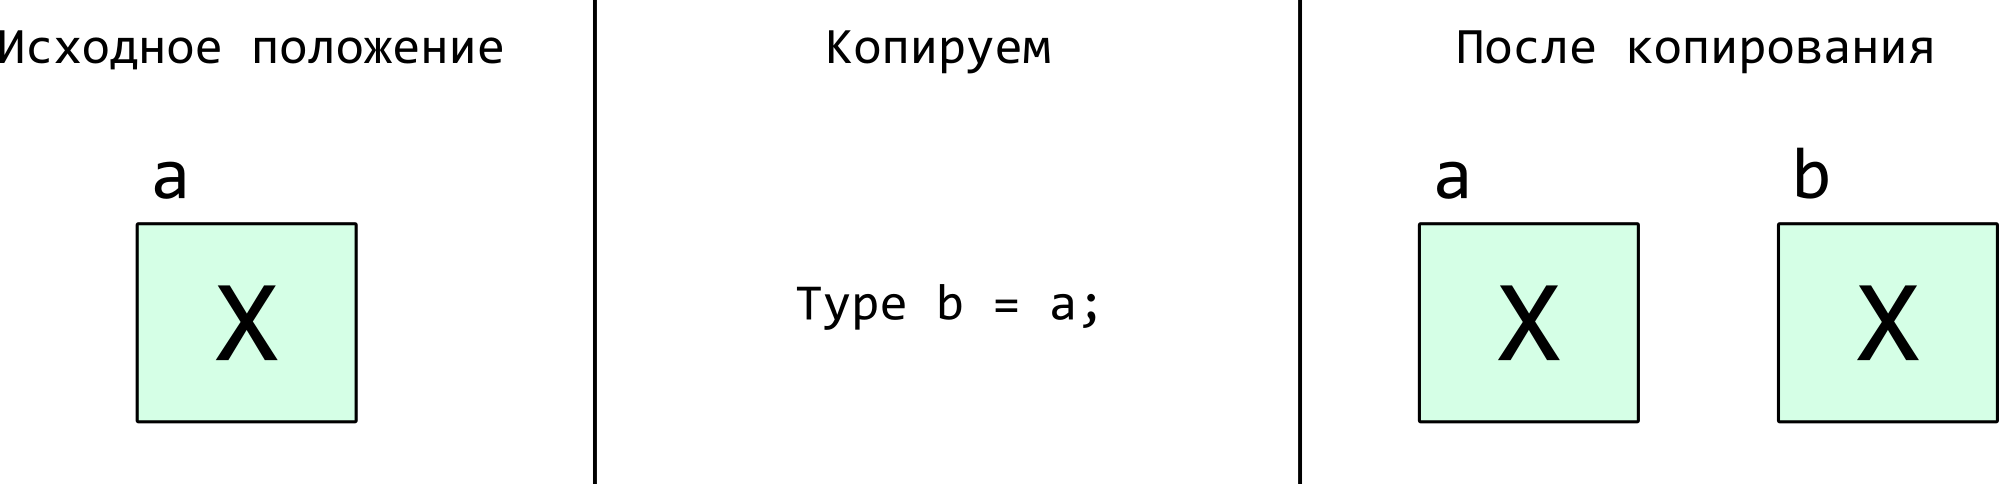
\includegraphics[scale=0.9]{../images/copy.png}
\end{center}
После копирования объект \texttt{b} будет находится в том же состоянии, что и \texttt{a}.

То, каким образом производится копирование, зависит от типа объекта:
\begin{itemize}
\item Если \texttt{Type} это скалярный тип, то происходит копирование байт из одного объекта в другой.
\item Если \texttt{Type} это класс, то вызывается конструктор копирования.
\item Если \texttt{Type} это агрегат, то операция копирования применяется к каждому элементу агрегата.
\end{itemize}



\subsection*{Операция перемещения}
Перемещаем \texttt{a} в новый объект \texttt{b}. Для этого используется стандартная функция \texttt{std::move}:
\begin{center}
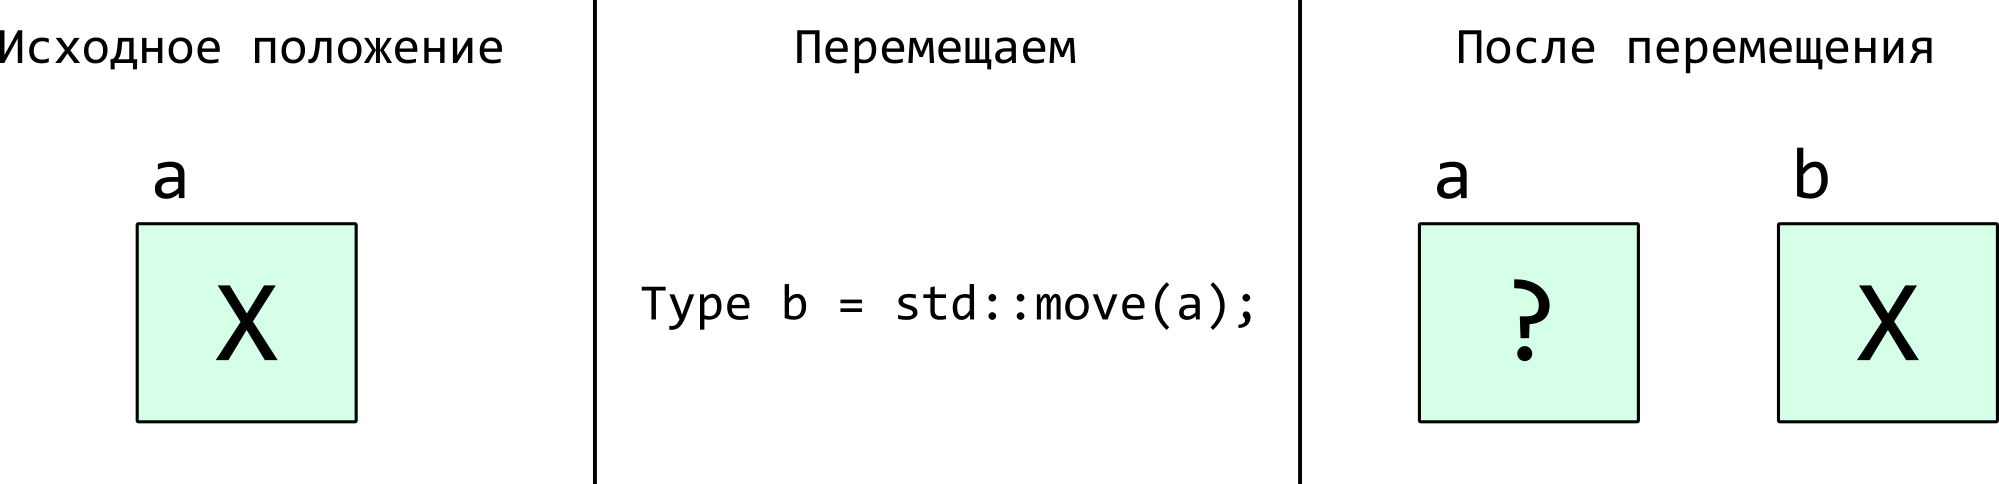
\includegraphics[scale=0.9]{../images/move.png}
\end{center}
После перемещения объект \texttt{b} будет находится в том состоянии, в котором объект \texttt{a} находился до перемещения. Но состояние объекта \texttt{a} может измениться на другое (на картинке это состояние отмечено значком вопроса). То, в каком состоянии окажется \texttt{a} после перемещения, различается для разных типов. Однако это состояние должно быть корректным. Это означает, что мы можем переиспользовать переменную \texttt{a} в дальнейшем.

То, каким образом производится перемещение, зависит от типа объекта:
\begin{itemize}
\item Если \texttt{Type} это скалярный тип, то происходит копирование байт из одного объекта в другой.
\item Если \texttt{Type} это класс, то вызывается конструктор перемещения (этот конструктор будет разобран позже). Конструктор перемещения может изменить объект из которого происходит перемещение. Если конструктора перемещения у этого класса нет, то вызывается конструктор копирования.
\item Если \texttt{Type} это агрегат, то операция перемещения применяется  к каждому элементу агрегата.
\end{itemize}





\newpage
\section*{Перемещение объектов различных типов}
\subsection*{Перемещение объектов скалярных типов}
\iffalse
При копировании объекта скалярного типа он просто копируется побайтово:\\
\noindent\begin{minipage}{.30\textwidth}
\begin{lstlisting}
int a = 123;
int b = a;
\end{lstlisting}
\end{minipage}\hfill
\begin{minipage}{.60\textwidth}
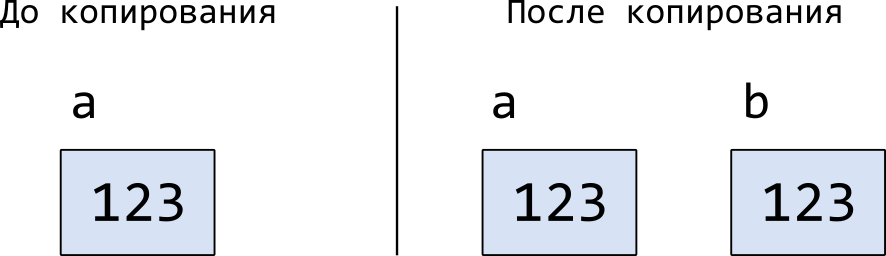
\includegraphics[scale=1]{../images/copy_int.png}
\end{minipage}
\quad\\
\quad\\
\fi

При перемещении объекта скалярного типа он копируется побайтово также как и при копировании. То есть, для скалярных типов нет никакой разницы между копированием и перемещением.\\

\noindent\begin{minipage}{.30\textwidth}
\begin{lstlisting}
int a = 123;
int b = std::move(a);
\end{lstlisting}
\end{minipage}\hfill
\begin{minipage}{.60\textwidth}
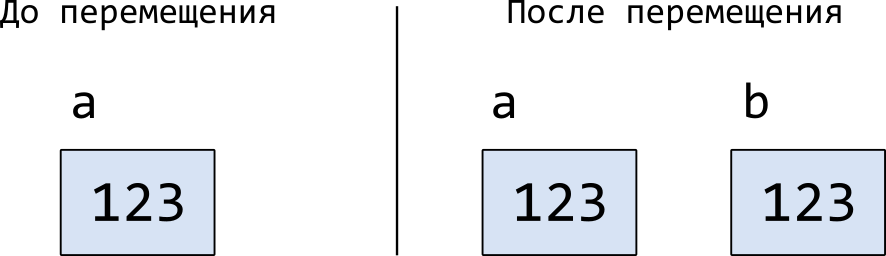
\includegraphics[scale=1]{../images/move_int.png}
\end{minipage}




\subsection*{Копирование вектора}
Так как вектор является классом, то, что происходит при копировании, задаётся в конструкторе копирования вектора. Конструктор копирования класса \texttt{std::vector} написан таким образом, чтобы при копировании происходило глубокое копирование вектора.
\begin{lstlisting}
std::vector<int> a {10, 20, 30};
a.reserve(5);
std::vector<int> b = a;
\end{lstlisting}

\begin{center}
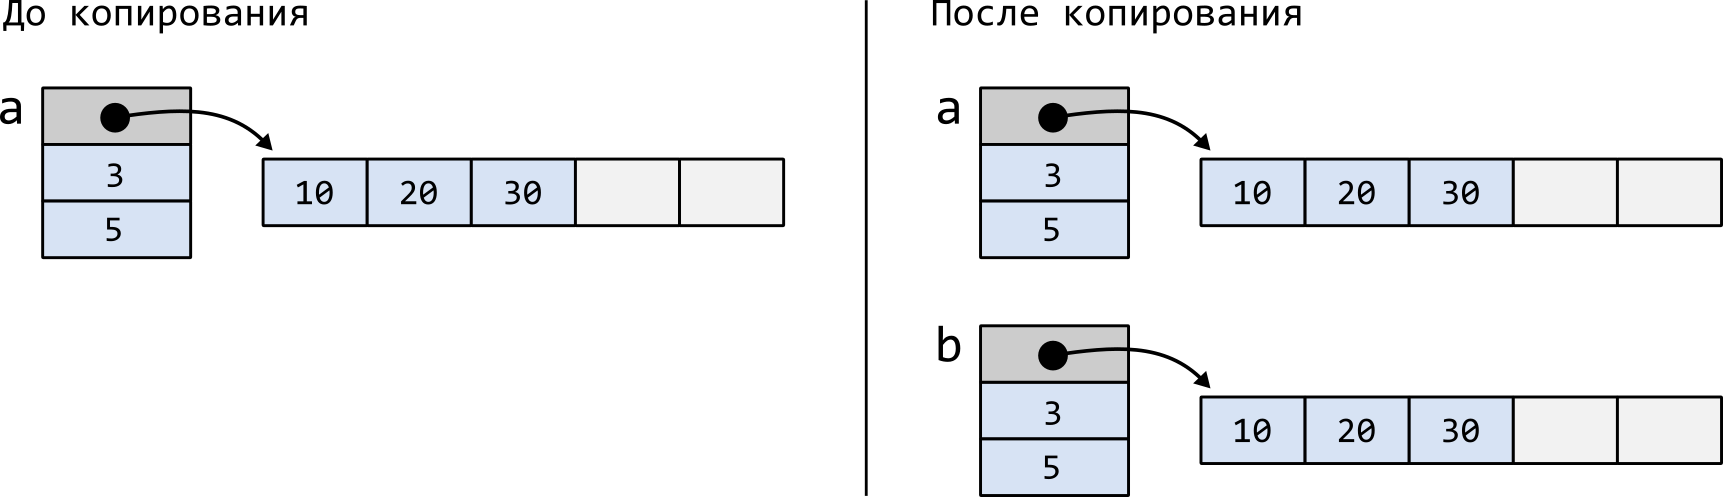
\includegraphics[scale=1]{../images/copy_vector.png}
\end{center}

\subsection*{Перемещение вектора}
Так как вектор является классом, то, что происходит при перемещении, задаётся в конструкторе перемещения. Конструктор перемещения вектора написан таким образом, чтобы при перемещении происходило следующее:
\begin{enumerate}
\item Поверхностное копирование (то есть копируется только сам объект вектора)
\item Зануление полей объекта, из которого производится перемещение.
\end{enumerate}
\begin{lstlisting}
std::vector<int> a {10, 20, 30};
a.reserve(5);
std::vector<int> b = std::move(a);
\end{lstlisting}
\begin{center}
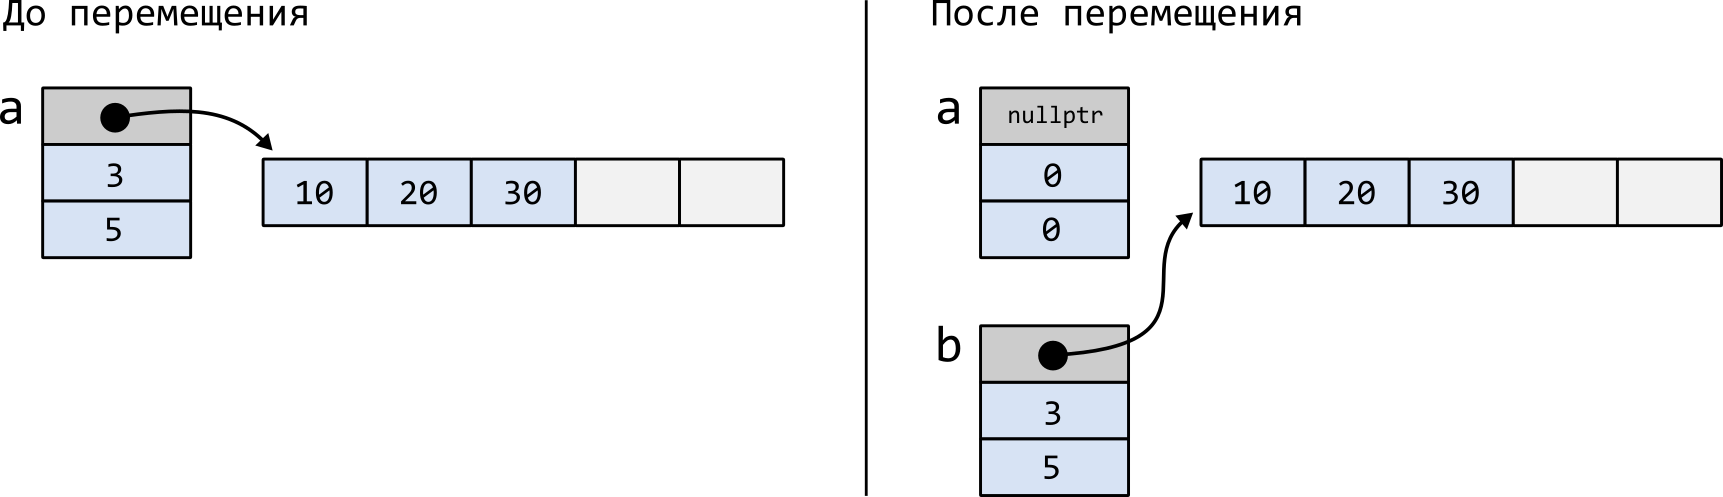
\includegraphics[scale=1]{../images/move_vector.png}
\end{center}
После перемещения вектор \texttt{a} становится пустым, но продолжает находиться в корректном состоянии. В него, например, можно скопировать или переместить другой вектор. Перемещение вектора намного более быстрая операция, чем его копирование, особенно для больших векторов.



\subsection*{Перемещение агрегатного типа \texttt{std::array<int>}}
Так как массив \texttt{std::array} является агрегатным типом, то при перемещении объекта этого типа, операция перемещения применяется к каждому элементу \texttt{std::array}. В данном случае типом элемента является скалярный тип \texttt{int}. Поэтому перемещение такого массива не будет отличаться от копирования.\\

\begin{minipage}{0.45\textwidth}
\begin{lstlisting}
std::array<int, 3> a {10, 20, 30};
std::array<int, 3> b = std::move(a);
\end{lstlisting}
\end{minipage}
\begin{minipage}{0.45\textwidth}
\begin{center}
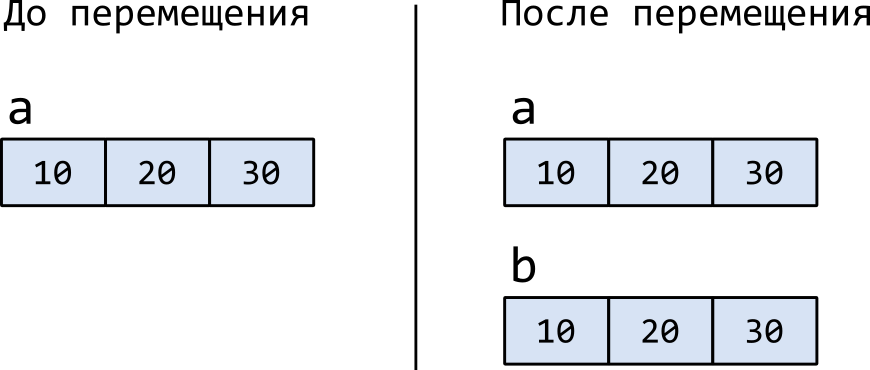
\includegraphics[scale=1]{../images/move_array_int.png}
\end{center}
\end{minipage}


\subsection*{Перемещение агрегатного типа \texttt{std::array<std::vector<int>{}>}}
В данном случае типом элемента агрегата является класс \texttt{std::vector<int>}. Поэтому перемещение объекта типа \texttt{\texttt{std::array<std::vector<int>{}>}} будет заключаться в перемещении каждого из векторов, находящися в массиве.
\begin{lstlisting}
using std::vector;
std::array<vector<int>, 3> a {vector{10, 20, 30}, vector{40, 50, 60, 70}, vector{80}};
std::array<vector<int>, 3> b = std::move(a);
\end{lstlisting}
\begin{center}
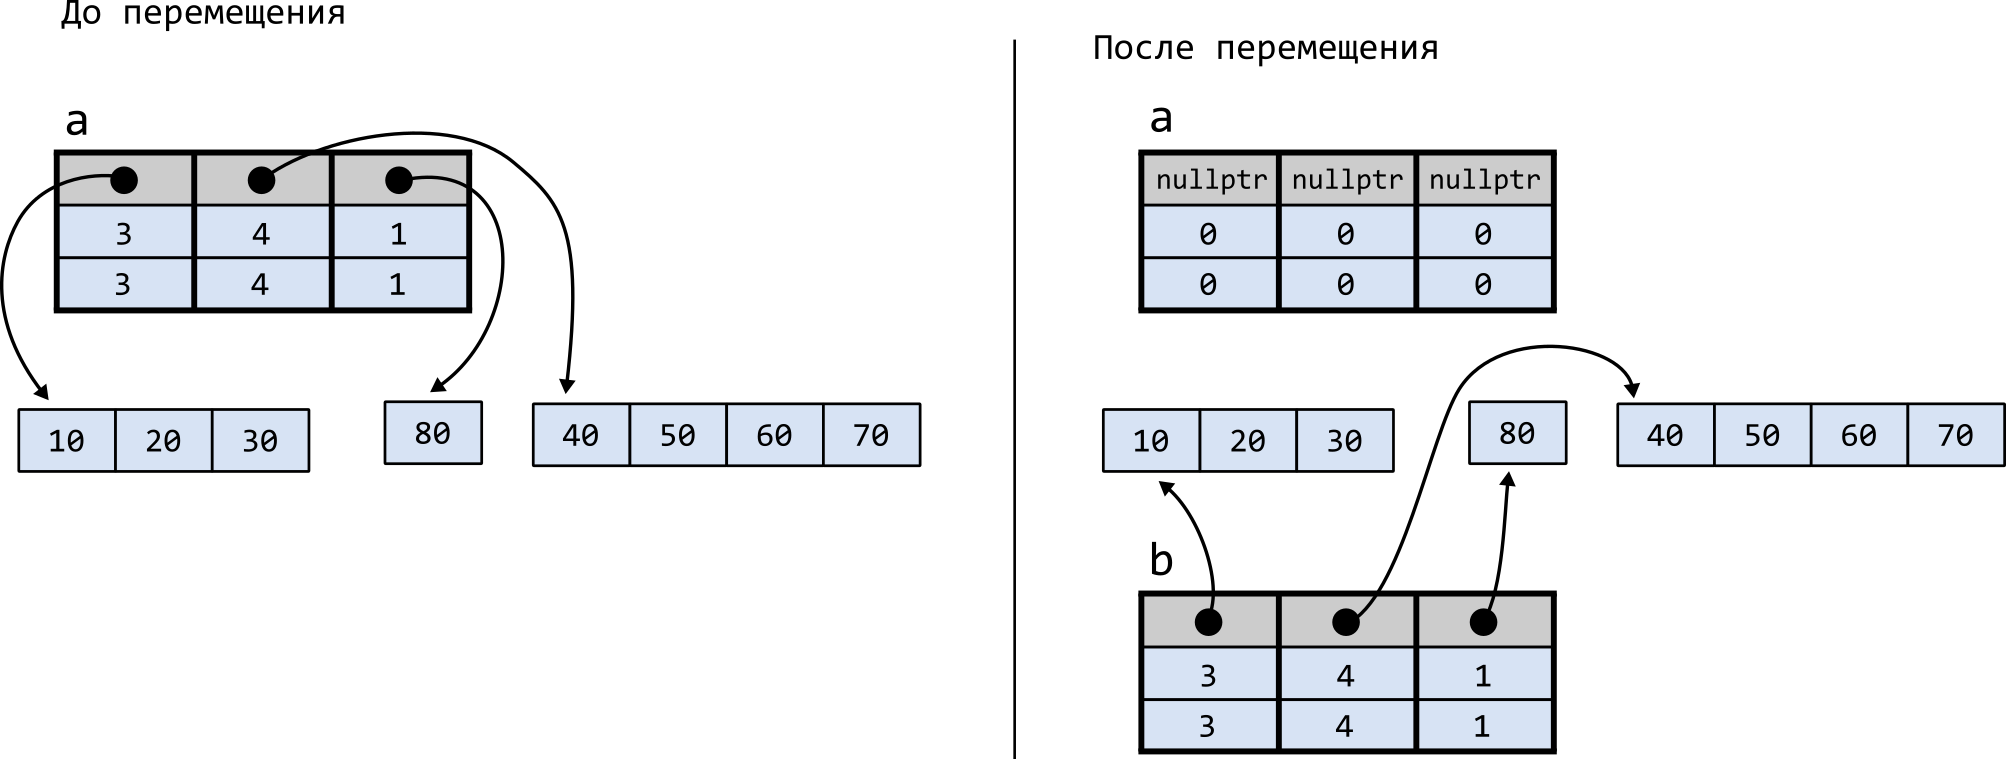
\includegraphics[scale=1]{../images/move_array_vector.png}
\end{center}


\subsection*{Перемещение длинной строки}
Длинная строка перемещается почти также, как и вектор. Перемещение длинной строки гораздо более эффективная операция, чем её копирование.
\begin{lstlisting}
std::string a = "The incredibly long string";
std::string b = std::move(a);
\end{lstlisting}
\begin{center}
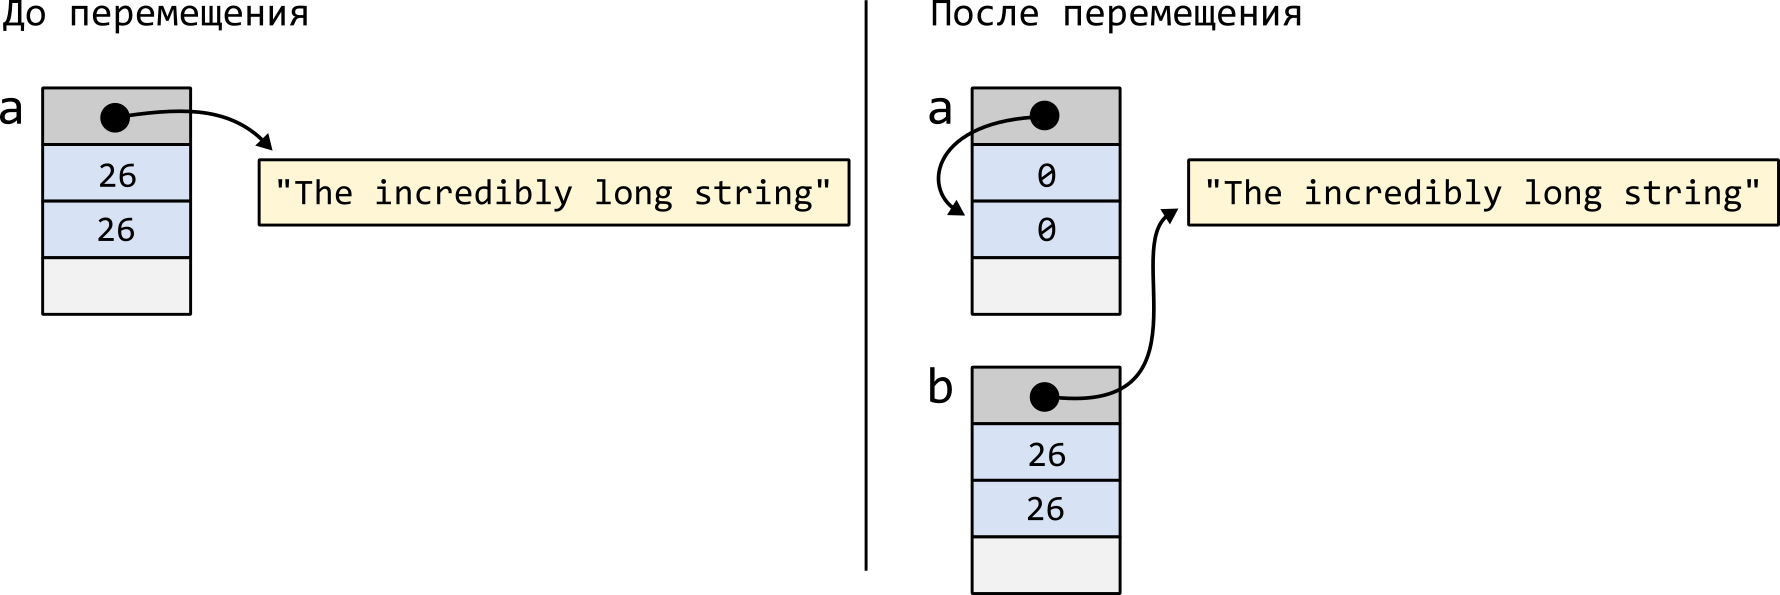
\includegraphics[scale=1]{../images/move_long_string.png}
\end{center}


\subsection*{Копирование короткой строки}
Интересен случай короткой строки. Из-за оптимизации малой строки (\textit{small string optimization}) строка в памяти имеет необычный вид -- одно из её полей является указателем, который указывает на другое полей. Копирование такой строки не совсем тривиально, так как указатель нужно задать правильным образом.\\

\quad\\
\begin{minipage}{0.4\textwidth}\noindent
\begin{lstlisting}
std::string a = "Short string";
std::string b = a;
\end{lstlisting}
\end{minipage}
\begin{minipage}{0.4\textwidth}
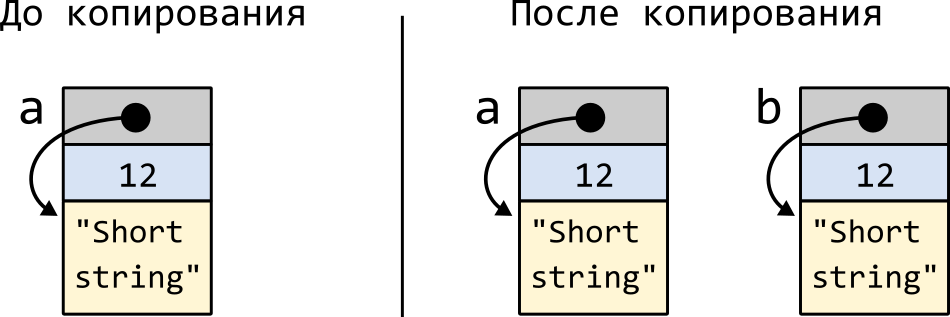
\includegraphics[scale=1]{../images/copy_short_string.png}
\end{minipage}


\subsection*{Перемещение короткой строки}
Перемещая короткую строку \texttt{a} мы создаём новую строку \texttt{b} тем же способом, что и при копировании. Однако после этого нам нужно ещё занулить начальную строку \texttt{a}, потому что мы хотим, чтобы поведение короткой строки при перемещении было согласовано с поведением длинной строки. Таким образом получается необычная ситуация, когда перемещение для короткой строки работает немного медленней, чем копирование.\\

\begin{minipage}{0.4\textwidth}\noindent
\begin{lstlisting}
std::string a = "Short string";
std::string b = std::move(a);
\end{lstlisting}
\end{minipage}
\begin{minipage}{0.4\textwidth}
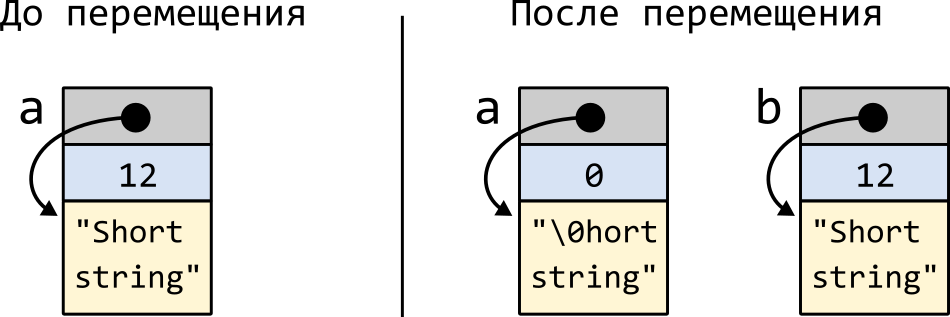
\includegraphics[scale=1]{../images/move_short_string.png}
\end{minipage}


\section*{Операция перемещающего присваивания}
Перемещение может происходить не только при создании нового объекта, но и при присваивании к уже существующему объекту. Это делается с помощью так называемой операции перемещающего присваивания. Пусть у нас есть объекты:
\begin{lstlisting}
Type a = X;
Type b = Y;
\end{lstlisting}
Рассмотрим, что будет происходить при перемещающем присваивании одного объекта другому:\\

\begin{center}
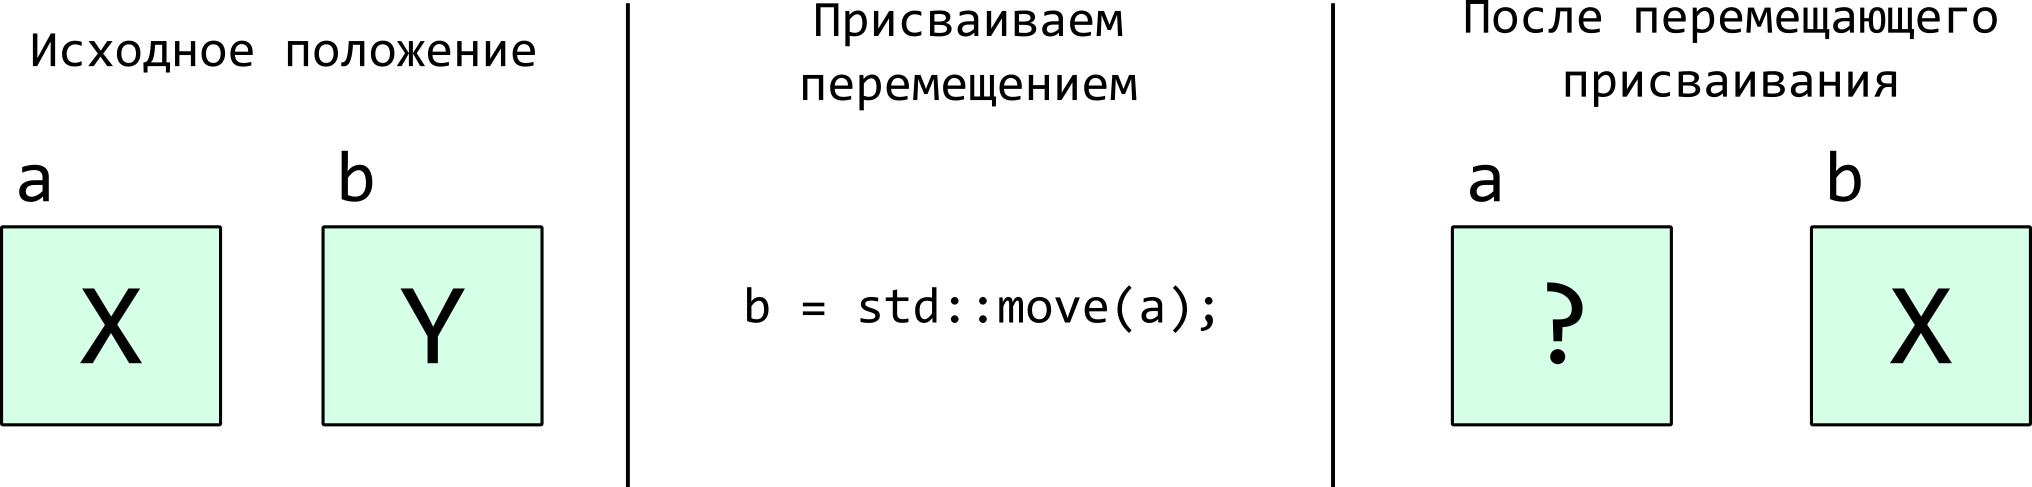
\includegraphics[scale=0.9]{../images/move_assignment.png}
\end{center}

То, каким образом производится перемещающее присваивание, зависит от типа объекта:
\begin{itemize}
\item Если \texttt{Type} это скалярный тип, то происходит копирование байт из одного объекта в другой.
\item Если \texttt{Type} это класс, то вызывается оператор присваивания перемещения (этот оператор будет разобран позже). Этот перегруженный оператор может изменить присваиваемый объект. Если оператора присваивания перемещения у этого класса нет, то вызывается оператор присваивания копирования (то есть обычнй оператор присваивания).
\item Если \texttt{Type} это агрегат, то операция перемещающего присваивания применяется к каждому его элементу.
\end{itemize}

\newpage
\section*{В каких случаях происходит перемещение}
\subsection*{Определение понятия "выражение"}
\textit{Выражение} (англ. \textit{expression}) -- это последовательность операторов и их операндов, которая определяет некоторое вычисление. Учтите, что существуют такие операторы, как оператор вызова функции (также известный как оператор круглые скобочки \texttt{()}), а также оператор индексирования (\texttt{[]}), оператор точка и стрелочка.\\
Поэтому, например, следующая последовательность является выражением:
\begin{lstlisting}
f(2 * a[i + 1]) + c.x / p->call()
\end{lstlisting}
Простейшими выражениями, являются выражения, состоящие из одного имени переменной или литерала. Например, \texttt{a} или \texttt{10} являются примерами простейших выражений.

\subsection*{Категории выражений}
Выражения можно поделить на две категории: lvalue и rvalue. Точное определение того что такое lvalue, а что такое rvalue тут пока не будет дано (так как это определение очень объёмно).
Но можно думать о категории выражения следующим образом:

\begin{itemize}
\item \textit{lvalue-выражения} или просто \textit{lvalue} -- это такие выражения, которые соответствуют какому-то объекту в памяти и у таких выражений можно получить адрес. Примеры таких выражений:
\begin{lstlisting}
a	arr[i]	   *p     arr[1 + func(a / b + c)]
\end{lstlisting}
\item \textit{rvalue-выражения} или просто \textit{rvalue} -- все остальные выражения.
Примеры таких выражений:
\begin{lstlisting}
10       a + 1     a * b       abs(a)     -a
\end{lstlisting}
\end{itemize}
Таким образом, любое выражение характеризуется двумя независимыми свойствами:
\begin{enumerate}
\item Тип выражения
\item Категория выражения: lvalue или rvalue
\end{enumerate}


\subsection*{Когда происходит перемещение}
Перемещение происходит в частности в следующих ситуациях:
\begin{enumerate}
\item При инициализации объекта rvalue-выражением:
\begin{lstlisting}
Type a = rvalue-expression;     
Type b{rvalue-expression}; 
Type c(rvalue-expression);
\end{lstlisting}
Рассмотрим пример:
\begin{lstlisting}
#include <iostream>
#include <string>
int main()
{
    std::string a{"Cat"};
    std::string b{"Mouse"};
    
    std::string c = a;      // Строка a скопируется в объект c, так как a это lvalue.
    
    std::string d = a + b;  // Сначала создастся временная строка a + b.
                            // Затем эта временная строка переместится в объект d.
                            // Компилятор поймёт, что в данном случае нужно перемещать,
                            // так как выражение a + b это rvalue.
}
\end{lstlisting}

\item При присваивании, если справа находится rvalue-выражение
\begin{lstlisting}
a = rvalue-expression;
\end{lstlisting}
Рассмотрим пример:
\begin{lstlisting}
#include <iostream>
#include <string>
int main()
{
    std::string a{"Cat"};
    std::string b{"Mouse"};
    std::string c;
    std::string d;
    
    c = a;          // Строка a скопируется в объект c, так как a это lvalue.
    
    d = a + b; 	    // Сначала создастся временная строка a + b.
                    // Затем эта временная строка переместится в объект d,
                    // так как a + b это rvalue.
}
\end{lstlisting}


\item При передаче rvalue-выражения в функцию, принимающую по значению:
\begin{lstlisting}
void func(Type x);
...
func(rvalue-expression);
\end{lstlisting}

Рассмотрим пример:
\begin{lstlisting}
#include <iostream>
#include <string>

void func(std::string x)
{
    std::cout << x << std::endl;
}
int main()
{
    std::string a{"Cat"};
    std::string b{"Mouse"};
    
    func(a);     // Строка a скопируется в функцию func, так как a - это lvalue
    func(a + b); // Временная строка a + b переместится в func, так как a + b - это rvalue
}
\end{lstlisting}


\end{enumerate}



\subsection*{Функция \texttt{std::move}}
Стандартная функция \texttt{std::move} из библиотеки \texttt{utility} на самом деле сама ничего никуда не перемещает. Эта функция просто преобразует lvalue-выражение в rvalue-выражение. То есть, если есть переменная \texttt{a}, то выражение \texttt{std::move(a)} является rvalue.
\begin{lstlisting}
void func(std::string x);
...
std::string a{"Cat"};
func(a);            // Строка a скопируется в функцию func, так как a - это lvalue
func(std::move(a)); // Строка a переместится в func, так как std::move(a) - это rvalue
                    // В данной ситуации мы перемещаем не временную строку, а именно строку a, 
                    // поэтому после этой операции строка a станет пустой.
\end{lstlisting}

\newpage



\newpage
\section*{Польза перемещения}
Перемещение очень полезно тогда, когда объект из которого производится перемещение перестаёт быть нужным после перемещения. В этих случаях перемещение позволяет существенно ускорить программу.
\subsection*{Перемещение временных объектов}
Рассмотрим следующий пример. Есть две строки \texttt{a} и \texttt{b}, которые потенциально могут быть очень длинными. Мы хотим конкатенировать эти строки и сохранить результат в другой строке \texttt{s}.
\begin{lstlisting}
s = a + b;
\end{lstlisting}
В этом случае будут произведены следующие операции:
\begin{enumerate}
\item Конкатенирование строки с помощью метода \texttt{operator+} строки. При этом создаётся некоторый временный объект (типа \texttt{std::string}), в котором будет хранится результат конкатенации.
\item Перемещение этого временного объекта в строку \texttt{s}.
\end{enumerate}
Без перемещения, на втором шаге нам бы пришлось копировать временный объект в строку \texttt{s}, что могло было быть намного менее эффективно.
Аналогично, перемещение ускоряет программу, когда мы передаём временные объект в функции по значению.
\begin{lstlisting}
void func(std::string s) {...};
// ...
func(a + b); // Тут используется перемещение
\end{lstlisting}

\subsection*{Ускорение некоторых операций с помощью перемещения}
Перемещение может быть полезно не только для временных объектов. Перемещая обычные невременные объекты можно ускорить многие алгоритмы. Рассмотрим, например, задачу обмена значений двух строк, которые потенциально могут быть очень длинными:
\begin{lstlisting}
std::swap(a, b);
\end{lstlisting}
Функция \texttt{swap} просто перемещает объекты и реализована следующим образом:
\begin{lstlisting}
template<typename T> 
void swap(T& a, T& b) 
{
    T temp = std::move(a);
    a = std::move(b);
    b = std::move(temp);
}
\end{lstlisting}
Без перемещения объекты пришлось бы многократно копировать внутри функции \texttt{swap}, что было бы очень неэффективно для объектов, владеющих памятью в куче. С перемещением \texttt{swap} работает намного быстрее для объектов, выделяющих память в куче. Соответственно, будут работать намного быстрее все алгоритмы, использующие \texttt{swap} (например, алгоритмы сортировки).

\subsection*{Возвращаемое значение функции}
Перемещение может помочь при возврате объекта из функции. Но в этом случае обычно нет необходимости использовать \texttt{std::move}, так как перемещение происходит автоматически. Более того, использование \texttt{std::move} может не дать компилятору использовать RVO(Return Value Optimization), что может даже привести к более медленному коду.


\newpage
\section*{Пример перемещения различных объектов в функций}
\begin{lstlisting}
#include <iostream>
#include <string>
#include <vector>
using std::cout, std::endl;
void func(int x)
{
    cout << "int inside func: " << x << endl;    
}

void func(std::string x)
{
    cout << "string inside func: " << x << endl;    
}

void print_vector(const std::vector<int>& v)
{
    cout << "( ";
    for (auto el : v)
        cout << el << " ";
    cout << ")" << endl;
}

void func(std::vector<int> x)
{
    cout << "vector inside func: "; 
    print_vector(x);   
}

int main()
{
    int a = 123;
    func(std::move(a));
    cout << "int after move: " << a << endl << endl;
    
    std::string b{"Cat"};
    func(std::move(b));
    cout << "string after move: " << b << endl << endl;
     
    std::vector<int> c{10, 20, 30};
    func(std::move(c)); 
    cout << "vector after move: ";
    print_vector(c);
}
\end{lstlisting}
Данная программа напечатает:
\begin{verbatim}
int inside func: 123
int after move: 123

string inside func: Cat
string after move:

vector inside func: ( 10 20 30 )
vector after move: ( )
\end{verbatim}




\section*{rvalue-ссылки}

\subsection*{Инициализация rvalue-ссылок}
Если функция принимает аргумент по значению, то при передаче в неё lvalue передаваемый объект копируется, а при передаче rvalue объект перемещается. Если же функция принимает аргумент по ссылке, то никакого копирования и перемещения не происходит, а в функции просто создаётся ссылка, на передаваемый объект. 

Для того, чтобы можно было различать категорию выражения при передаче по ссылке в язык были введены \texttt{rvalue}-ссылки. Тип rvalue-ссылки состоит из названия типа с двумя амперсандами на конце:
\begin{lstlisting}
int& l;   -  это lvalue - ссылка на int
int&& r;  -  это rvalue - ссылка на int
\end{lstlisting}
rvalue-ссылки очень похожи на обычные ссылки (также известные как lvalue-ссылки). Одно из двух отличий rvalue-ссылок от lvalue-ссылок заключается в том, что первые инициализируются только \texttt{rvalue}-выражениями.
\lstset{literate=%
   *{0}{{{\color{red!20!violet}0}}}1
    {1}{{{\color{black}1}}}1
    {2}{{{\color{black}2}}}1
    {3}{{{\color{black}3}}}1
    {4}{{{\color{red!20!violet}4}}}1
    {5}{{{\color{red!20!violet}5}}}1
    {6}{{{\color{red!20!violet}6}}}1
    {7}{{{\color{red!20!violet}7}}}1
    {8}{{{\color{red!20!violet}8}}}1
    {9}{{{\color{red!20!violet}9}}}1
}
\begin{lstlisting}
int a = 50;

int& l1 = a;        // OK, lvalue - ссылка инициализируется lvalue - выражением
int& l2 = a + 1;    // Error, lvalue - ссылка не может инициализироваться rvalue - выражением

int&& r1 = a;       // Error, rvalue - ссылка не может инициализироваться lvalue - выражением
int&& r2 = a + 1;   // OK, rvalue - ссылка инициализируется rvalue - выражением
int&& r3 = r2;      // Error, r2 - это lvalue выражение

r2 += 5;            // С rvalue - ссылками можно работать также, как и с обычными ссылками
cout << r2 << endl; // Напечатает 56
\end{lstlisting}


\subsection*{Перегрузка по категории выражения}
С помощью \texttt{rvalue} ссылок и перегрузки функций можно различить категорию выражения, приходящую на вход функции. В примере вызовется соответствующий вариант перегрузки в зависимости от категории выражения.
\begin{lstlisting}
#include <iostream>
#include <string>

void func(std::string& s)
{
    std::cout << "lvalue" << std::endl;
}

void func(std::string&& s)
{
    std::cout << "rvalue" << std::endl;
}
int main() 
{
    std::string a = "Cat";
    std::string b = "Dog";

    func(a);               // Передадим по lvalue ссылке
    func(a + b);           // Передадим по rvalue ссылке
    func(std::move(a));    // Передадим по rvalue ссылке
    std::cout << "a = " << a << std::endl;  // Напечатает Cat
    std::cout << "b = " << b << std::endl;  // Напечатает Dog
}
\end{lstlisting}
Обратите внимание, что в этом примере никакого копирования и перемещения происходить не будет вообще, так как обе функции принимают аргументы по ссылке.



\subsection*{Константные lvalue-ссылки и rvalue-выражения}
Константные lvalue-ссылки обладают неочевидным свойством -- они могут инициализироваться как lvalue так и rvalue выражениями. То есть можно написать так:
\begin{lstlisting}
int a = 50;
const int& cl = a + 1;  // OK, может инициализироваться rvalue
\end{lstlisting}
Все возможные варианты инициализации ссылок представлены в следующем примере:
\begin{lstlisting}
int a = 50;
const int b = 500;

int& l1 = a;            // OK
int& l2 = b;            // Error, так как b - это константа
int& l3 = a + 1;        // Error, так как a + 1 - это rvalue

const int& c1 = a;      // OK
const int& c2 = b;      // OK
const int& c3 = a + 1;  // OK

int&& r1 = a;           // Error, так как a - это lvalue
int&& r2 = b;           // Error, так как b - это константа и lvalue
int&& r3 = a + 1;       // OK
\end{lstlisting}


\subsection*{Перегрузка между rvalue-ссылкой и константной lvalue-ссылкой}
Удобно делать перегрузку между rvalue-ссылкой и константной lvalue-ссылкой.
В этом случае, если мы передадим rvalue, подойдут обе функции, но по правилам перегрузки выберется перегрузка с rvalue-ссылкой. Удобство такой перегрузки заключается в том, что lvalue-выражения будут приниматься по константной ссылке (что хорошо, так как мы обычно не хотим менять существующий объект), в rvalue-выражения будут приниматься по неконстантной ссылке (что тоже хорошо, так как часто нужно изменить такой объект).
\begin{lstlisting}
#include <iostream>
#include <string>

void func(const std::string& s)
{
    std::cout << "const lvalue ref" << std::endl;
}

void func(std::string&& s)
{
    std::cout << "rvalue ref" << std::endl;
}

int main() 
{
    std::string a = "Cat";
    std::string b = "Dog";

    func(a);               // Подходит только const lvalue ref
    func(a + b);           // Подходят обе функции, но выберется rvalue ref
    func(std::move(a));    // Подходят обе функции, но выберется rvalue ref
}
\end{lstlisting}

\newpage
\subsection*{Возврат rvalue-ссылок из функций}
Второе и последнее отличие rvalue-ссылок от обычных lvalue-ссылок проявляется при возврате ссылок из функции или при приведении к типу ссылки.
\begin{itemize}
\item При возврате из функции lvalue-ссылки -- выражение вызовы функции будет lvalue-выражением.
\item При возврате из функции rvalue-ссылки -- выражение вызовы функции будет rvalue-выражением.
\end{itemize}
Это различие виндно на следующем примере:
\begin{lstlisting}
#include <iostream>
#include <string>

void printCategory(int& x)  {std::cout << "lvalue" << std::endl;}
void printCategory(int&& x) {std::cout << "rvalue" << std::endl;}

int a = 123;

int funcValue() {return a;}
int& funcLRef() {return a;}
int&& funcRRef(){return std::move(a);}

int main() 
{
    printCategory(funcValue());  // Напечатает rvalue
    printCategory(funcLRef());   // Напечатает lvalue
    printCategory(funcRRef());   // Напечатает rvalue
}
\end{lstlisting}

\subsection*{Приведение к lvalue/rvalue ссылкам}
Аналогичные правила приведению к типу ссылки:
\begin{lstlisting}
#include <iostream>
#include <string>

void printCategory(int& x)  {std::cout << "lvalue" << std::endl;}
void printCategory(int&& x) {std::cout << "rvalue" << std::endl;}

int main() 
{
    int a = 123;
    printCategory(static_cast<int&>(a));    // Напечатает lvalue
    printCategory(static_cast<int&&>(a));   // Напечатает rvalue
    
    int& l = a;
    printCategory(static_cast<int&&>(l));   // Напечатает rvalue
}
\end{lstlisting}
Используя это свойство можно написать простейшую реализацую функции \texttt{move}:
\begin{lstlisting}
template <typename T>
T&& mymove(T& x)
{
    return static_cast<T&&>(x);
}
\end{lstlisting}
Эта реализация не совсем правильная, так как она не может принимать на вход \texttt{rvalue}, но она всё-равно может дать понимание как работает функция \texttt{std::move}.

\newpage
\section*{Конструктор перемещения и оператор присваивания перемещения}
\subsection*{Конструктор перемещения для строки \texttt{String(String\&\& s) }}
\begin{lstlisting}
#include <cstring>
#include <iostream>
using std::cout, std::endl;

class String 
{
private:
    char* data;
    size_t size;
    size_t capacity;
public:
    String(const char* str) 
    {
        std::cout << "Constructor from C string\n";
        size = std::strlen(str);
        capacity = size;
        data = new char[capacity + 1];
        std::memcpy(data, str, size);
        data[size] = '\0';
    }

    String(const String& s)
    {
        std::cout << "Copy Constructor\n";
        size = s.size;
        capacity = s.capacity;
        data = new char[capacity + 1];
        std::memcpy(data, s.data, size);
        data[size] = '\0';
    }
    
    String(String&& s) 
    : data(s.data), size(s.size), capacity(s.capacity)
    {
        std::cout << "Move Constructor\n";
        
        s.data = nullptr;
        s.size = 0;
        s.capacity = 0;
    }
    ~String() {if (data) delete [] data;}  
    
    friend std::ostream& operator<<(std::ostream& out, const String& s);
};

std::ostream& operator<<(std::ostream& out, const String& s)
{
    if (s.data)
        out << s.data;
    return out;
}

int main()
{
    String a = "Cat";
    String b = a;              // Наша строка копируется, используя  String(const String& s)
    String c = std::move(a);   // Наша строка перемещается, используя  String(String&& s)
    
    cout << "a: " << a << endl;
    cout << "b: " << b << endl;
    cout << "c: " << c << endl;
}
\end{lstlisting}

\subsection*{Оператор присваивания перемещения для строки \texttt{String\& operator=(String\&\& s)}}
\begin{lstlisting}
#include <cstring>
#include <iostream>
using std::cout, std::endl;

class String 
{
private:
    char* data;
    size_t size;
    size_t capacity;
public:
    String(const char* str) 
    {
        std::cout << "Constructor from C string\n";
        size = std::strlen(str);
        capacity = size;
        data = new char[capacity + 1];
        std::memcpy(data, str, size);
        data[size] = '\0';
    }

    String(const String& s)
    {
        std::cout << "Copy Constructor\n";
        size = s.size;
        capacity = s.capacity;
        data = new char[capacity + 1];
        std::memcpy(data, s.data, size);
        data[size] = '\0';
    }
    
    String(String&& s) 
        : data(s.data), size(s.size), capacity(s.capacity)
    {
        std::cout << "Move Constructor\n";
        
        s.data = nullptr;
        s.size = 0;
        s.capacity = 0;
    }
    
    String& operator=(const String& s)
    {
        std::cout << "Copy Assignment\n";
        
        if (this == &s)
            return *this;

        size = s.size;
        capacity = s.capacity;

        std::free(data);
        data = new char[capacity + 1];
        std::memcpy(data, s.data, size + 1);

        return *this;
    }
    
    String& operator=(String&& s)
    {
        std::cout << "Move Assignment\n";
        
        if (this == &s)
            return *this;
        
        delete [] data;
        data = s.data;
        size = s.size;
        capacity = s.capacity;

        s.data = nullptr;
        s.size = 0;
        s.capacity = 0;

        return *this;
    }
    
    
    ~String() {if (data) delete [] data;}  
    
    friend std::ostream& operator<<(std::ostream& out, const String& s);
};

std::ostream& operator<<(std::ostream& out, const String& s)
{
    if (s.data)
        out << s.data;
    return out;
}

int main()
{
    String x = "Elephant";
    String y = "Dog";
    
    y = std::move(x);
    cout << "x: " << x << endl;
    cout << "y: " << y << endl;
}
\end{lstlisting}

\iffalse
\newpage
\section*{Часть 4: Умный указатель \texttt{std::unique\_ptr}}

\newpage
\section*{Часть 5: Умный указатель \texttt{std::shared\_ptr}}
\fi

\newpage
\section*{Глубокое и поверхностное копирование}
Во многих языках программирования существуют понятия глубокого и поверхностного копирования (deep copy и shallow copy). Под глубоким копированием понимается рекурсивное копирование объекта и всех ресурсов, связанных с ним (например, памяти, выделенной в куче). Как правило, \texttt{operator=} в языке C++ перегружается таким образом, чтобы проводить глубокое копирование.
\begin{center}
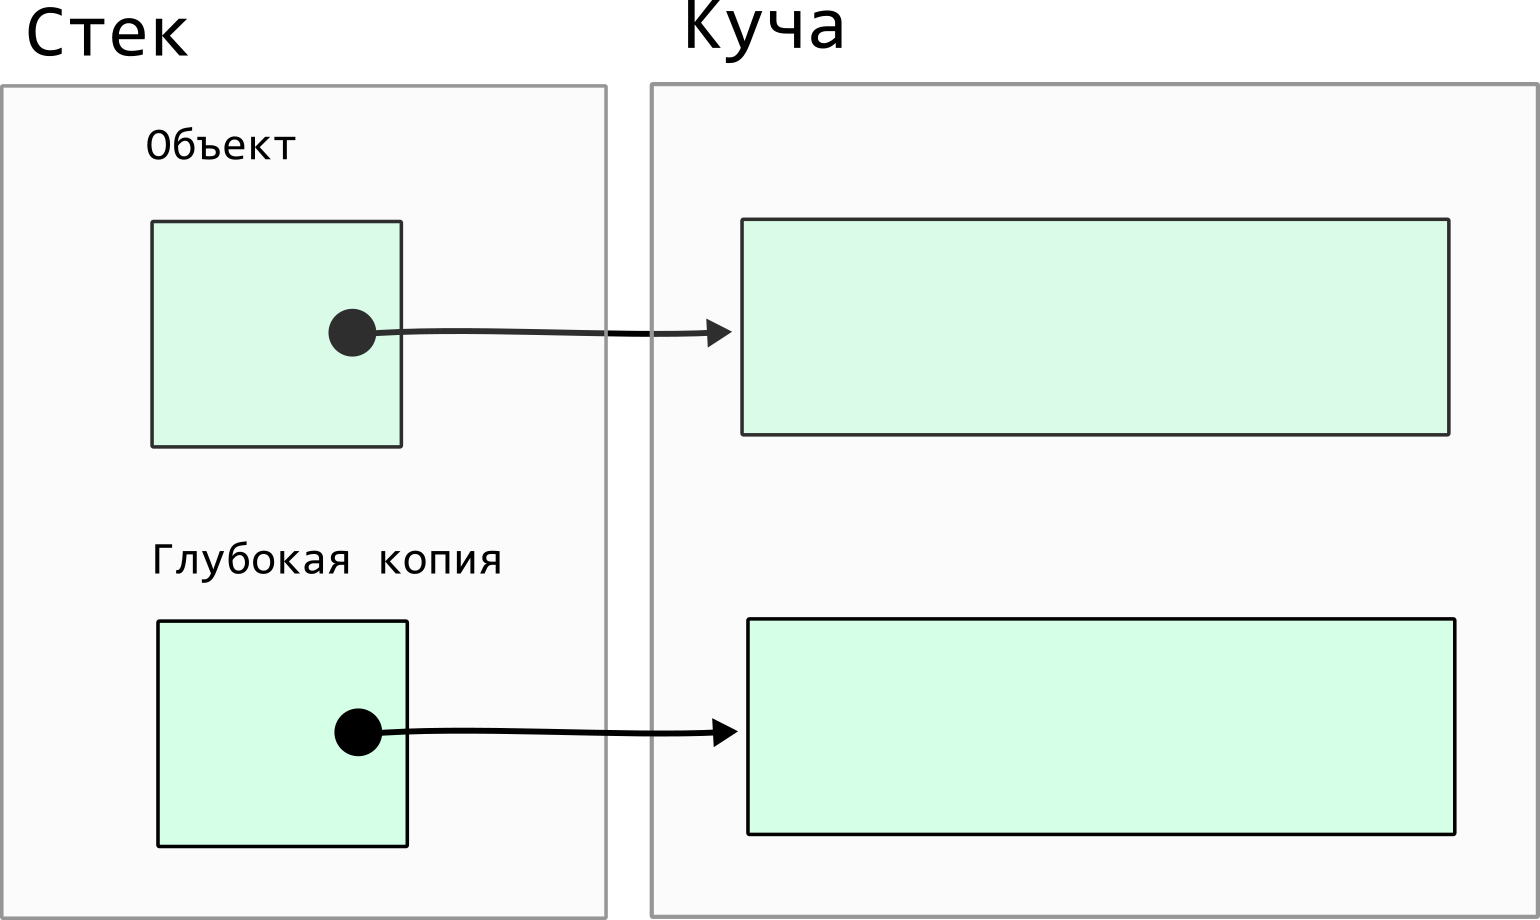
\includegraphics[scale=0.9]{../images/deep.png}
\end{center}

При поверхностном копировании происходит только побайтовое копирование полей объекта. В том числе копируются все указатели, которые продолжают указывать на ту же область памяти в куче. Так, например, работает присваивание структур в языке C.

\begin{center}
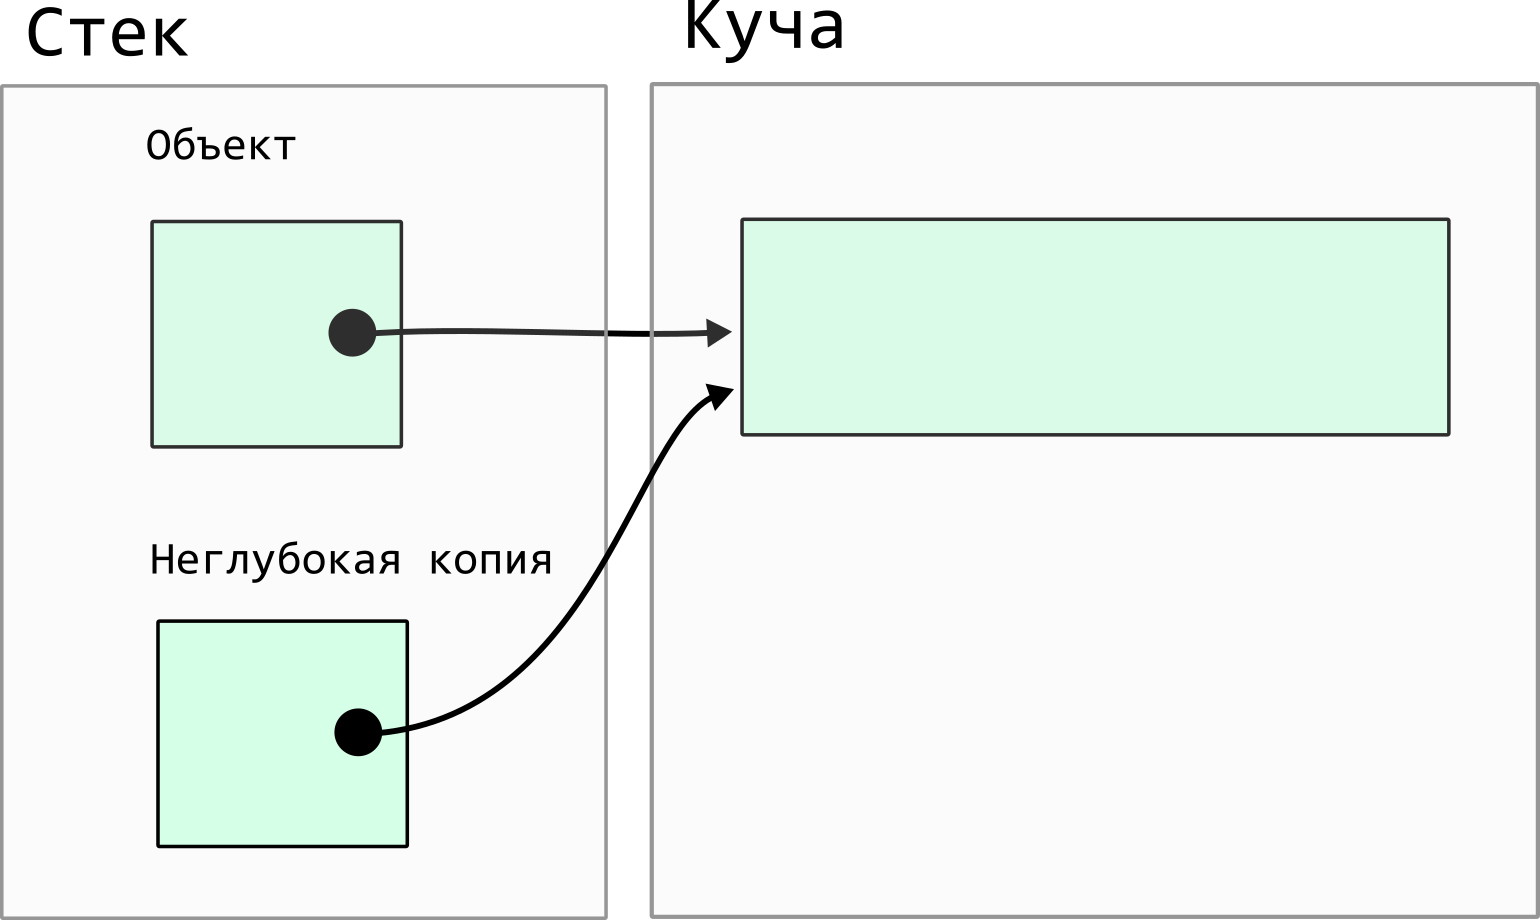
\includegraphics[scale=0.9]{../images/shallow.png}
\end{center}

Поверхностное копирование имеет множество недостатков, связанных с безопастностью работы программы. Более того, иногда нам нужна полная копия объекта и поверхностное копирование просто не подойдёт. Но есть и большое преимущество такого копирования -- оно значительно более эффективно.

\end{document}